%%%%%%%%%%%%%%%%%%%%%%%%%%%%%%%%%%%%%%%%%
% Structured General Purpose Assignment
% LaTeX Template
%
% This template has been downloaded from:
% http://www.latextemplates.com
%
% Original author:
% Ted Pavlic (http://www.tedpavlic.com)
%
% Note:
% The \lipsum[#] commands throughout this template generate dummy text
% to fill the template out. These commands should all be removed when
% writing assignment content.
%
%%%%%%%%%%%%%%%%%%%%%%%%%%%%%%%%%%%%%%%%%

%----------------------------------------------------------------------------------------
%	PACKAGES AND OTHER DOCUMENT CONFIGURATIONS
%----------------------------------------------------------------------------------------

\documentclass{article}
\setcounter{tocdepth}{4}
\setcounter{secnumdepth}{4}
\usepackage{fancyhdr} % Required for custom headers
\usepackage{lastpage} % Required to determine the last page for the footer
\usepackage{extramarks} % Required for headers and footers
\usepackage{graphicx} % Required to insert images
\usepackage{lipsum} % Used for inserting dummy 'Lorem ipsum' text into the template
\usepackage{url}
\usepackage{amsmath}
\usepackage{amssymb}
\usepackage{arydshln}
\usepackage{mathtools}
\usepackage{breqn}
\usepackage{fixltx2e}
\usepackage{indentfirst} 
\graphicspath{ {images/} }

% Margins
\topmargin=-0.45in
\evensidemargin=0in
\oddsidemargin=0in
\textwidth=6.5in
\textheight=9.0in
\headsep=0.25in

\linespread{1.1} % Line spacing

% Set up the header and footer
\pagestyle{fancy}
\lhead{\hmwkClass\ : \hmwkTitle} % Top center header
\rhead{\firstxmark} % Top right header
\lfoot{\lastxmark} % Bottom left footer
\cfoot{} % Bottom center footer
\rfoot{Page\ \thepage\ } % Bottom right footer
\renewcommand\headrulewidth{0.4pt} % Size of the header rule
\renewcommand\footrulewidth{0.4pt} % Size of the footer rule

\setlength\parindent{2em} % Indentation for paragraphs


%----------------------------------------------------------------------------------------
%	NAME AND CLASS SECTION
%----------------------------------------------------------------------------------------

\newcommand{\hmwkTitle}{Kalman Filtering for an Inverted Pendulum Final Report} % Assignment title
\newcommand{\hmwkDueDate}{Wednesday,\ June\ 6,\ 2018} % Due date
\newcommand{\hmwkClass}{MAE\ 298} % Course/class
\newcommand{\hmwkClassTime}{} % Class/lecture time
\newcommand{\hmwkClassInstructor}{Professor Lin} % Teacher/lecturer
\newcommand{\hmwkAuthorName}{Jordan McCrone, Sarah O'Meara, Peng Chen} % Your name

%----------------------------------------------------------------------------------------
%	TITLE PAGE
%----------------------------------------------------------------------------------------

\title{
\vspace{2in}
\textmd{\textbf{\hmwkClass:\ \hmwkTitle}}\\
\normalsize\vspace{0.1in}\large{Due\ on\ \hmwkDueDate}\\
\vspace{0.1in}\large{\textit{\hmwkClassInstructor\ \hmwkClassTime}}
\vspace{3in}
}

\author{\textbf{\hmwkAuthorName}}
\date{} % Insert date here if you want it to appear below your name

%----------------------------------------------------------------------------------------

\begin{document}

\maketitle

%----------------------------------------------------------------------------------------
%	TABLE OF CONTENTS
%----------------------------------------------------------------------------------------

%\setcounter{tocdepth}{1} % Uncomment this line if you don't want subsections listed in the ToC

\newpage
\tableofcontents
\listoffigures
\listoftables
\newpage

\section{Examples}
Test as seen in \cite{kane}

Example superscript JACO\textsuperscript{2} Example citation \cite{weisz2017assistive}

\begin{figure}[h!]
	\centering
	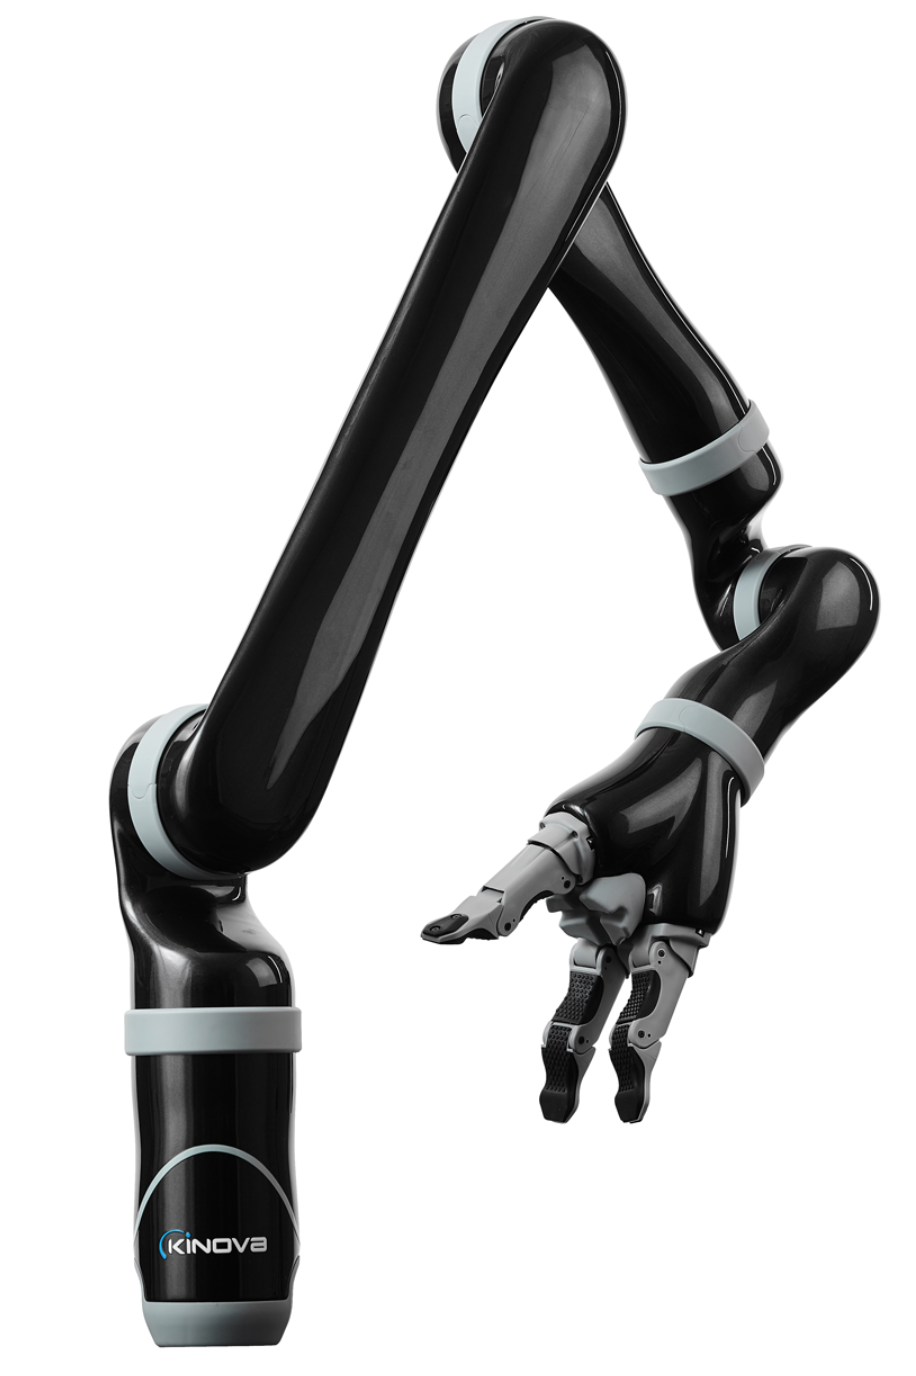
\includegraphics[width=5cm,keepaspectratio]{kinova.png}
	\caption{JACO\textsuperscript{2} 6-DOF Manipulator}
	\label{fig:diagram1}
\end{figure}

Example Figure \ref{fig:diagram1} Example symbols $\epsilon$. Example table

\begin{table}[h!]
\centering
\begin{tabular}{ |c |c  |c |c |c  |c  |c |}
\hline
	 i & 1 & 2 & 3 & 4 & 5 & 6 \\ \hline
	 a\textsubscript{i} & 0 & d\textsubscript{2} & 0 & 0 & 0 & 0 \\ \hline
	 $\alpha$\textsubscript{i}  & -90 & 0 & -90 & 90 & -90 & 0 \\ \hline
	 $\theta$\textsubscript{i} & $\theta$\textsubscript{1} & $\theta$\textsubscript{2} & $\theta$\textsubscript{3} & $\theta$\textsubscript{4} & $\theta$\textsubscript{5} & $\theta$\textsubscript{6} \\ \hline
	 s\textsubscript{i} & -d\textsubscript{1} & 0 & $\epsilon$\ &  d\textsubscript{3} + d\textsubscript{4} & 0 & d\textsubscript{5} + d\textsubscript{6} \\ \hline
\end{tabular}
\caption{D-H Parameters}
\label{table:1}
\end{table}

Example matrix with no equation number
\[
A_{1} = 
\begin{bmatrix}
	C\theta_{1} & 0 & -S\theta_{1} & 0 \\
	S\theta_{1} & 0 & C\theta_{1} & 0  \\
	0 & -1 & 0 & -d_{1} \\
	0 & 0 & 0 & 1 \\ 
\end{bmatrix}
\]

\section{Introduction}

 The inverted pendulum is a common system that has been well-studied in dynamics and controls.  The identifying characteristic of these systems is that the center of mass is above the pivot point resulting in an inherently unstable system.  Examples of inverted pendulum systems range from humans, where the feet are considered the pivot point, to the self-balancing Segway.  These systems are nonlinear and require a feedback control loop and state estimation in order to balance or stabilize the system, such that the center of mass remains directly above the pivot point.  Any displacement from this configuration will result in the center of mass moving to a new equilibrium at the lowest potential energy.  The center of mass can be repositioned above the pivot point by a control system that applies a restorative force.  It is critical to provide the controller with accurate state estimations in order to calculate the appropriate restorative force.  Inaccurate state estimation can destabilize the system leading to large oscillations or an undesirable state, such as the Segway falling onto the ground.

 This project used a pole on a cart model as an inverted pendulum system and investigated the use of different estimators: the Kalman Filter (KF), the Extended Kalman Filter, and the Unscented Kalman Filter.  Since the KF is used for linearized systems, it is hypothesized that its performance will degrade at larger angles as the small angle approximation will be used to linearize the equations of motion.  The project also tested the use of a single sensor and two sensors, and it is expected that two sensors will yield a more accurate estimation of the states.  Finally, this project evaluated the RMSE (root mean square error) and run time across estimators (KF, EKF, UKF) with different tuning.  The following sections discuss the system, state space models, test cases, results, and conclusions.

\section{Derivation of Continuous State Space Model}
\subsection{Description of System and Assumptions}
\subsection{System Parameters}

\begin{equation}
\textbf{x} = 
\begin{bmatrix}
	x \\
	\dot{x} \\
	\theta \\
	\dot{\theta} \\
\end{bmatrix}
\label{xMatrix}
\end{equation}

\begin{equation}
\beta = \dfrac{4}{3} - \dfrac{m}{M+m}
\end{equation}

\begin{equation}
\textbf{A} = 
\begin{bmatrix}
	1 & \tau & 0 & 0 \\
	0 & 1 & \dfrac{-gm\tau}{(M+m)\beta} & 0 \\
	0 & 0 & 1 & \tau \\
	0 & 0 & \dfrac{g\tau}{l\beta} & 1 \\
\end{bmatrix}
\label{aMatrix}
\end{equation}

\begin{equation}
\textbf{A} = 
\begin{bmatrix}
	1 & \tau & 0 & 0 \\
	0 & 1 & \dfrac{-gm\tau}{(M+m)\beta} & 0 \\
	0 & 0 & 1 & \tau \\
	0 & 0 & \dfrac{g\tau}{l\beta} & 1 \\
\end{bmatrix}
\label{aMatrix}
\end{equation}

\section{Estimators and Resulting Discretized State Space Models}
\subsection{Kalman Filter (KF)}
\subsection{Extended Kalman Filter (EKF)}
\subsection{Unscented Kalman Filter (UKF)}

\section{Methodology}

\section{Results}
\subsection{Offline Results}
\subsection{Online Results}

\section{Conclusions}

\section{References}

%\cite{*}
\bibliography{references}{}
\bibliographystyle{ieeetr}

\pagebreak
\section{Appendices}

\begin{dmath}
	\hat{z_{6}} \times \vec{r_{6}} = \left[\begin{matrix}0\\0\\0\end{matrix}\right]
\end{dmath}


\end{document}
